% Performance Impact Analysis of Intrusion Detection Systems on Windows 11
% !TeX spellcheck = en-US
% LTeX: language=en-US
% !TeX encoding = utf8
% !TeX program = lualatex
% !BIB program = bibtex

\documentclass[runningheads,a4paper,english]{llncs}[2022/01/12]

\usepackage{iftex}
\usepackage{upquote}
\usepackage[ngerman,main=english]{babel}
\addto\extrasenglish{\languageshorthands{ngerman}\useshorthands{"}}
\usepackage[hyphens]{url}

\makeatletter
\g@addto@macro{\UrlBreaks}{\UrlOrds}
\makeatother

\ifluatex
  \usepackage[no-math]{fontspec}
  \usepackage{unicode-math}
  \setmainfont[
    ItalicFont=NewCM10-Italic.otf,
    BoldFont=NewCM10-Bold.otf,
    BoldItalicFont=NewCM10-BoldItalic.otf,
    SmallCapsFeatures={Numbers=OldStyle}]{NewCM10-Regular.otf}
  \setsansfont[
    ItalicFont=NewCMSans10-Oblique.otf,
    BoldFont=NewCMSans10-Bold.otf,
    BoldItalicFont=NewCMSans10-BoldOblique.otf,
    SmallCapsFeatures={Numbers=OldStyle}]{NewCMSans10-Regular.otf}
  \setmonofont[ItalicFont=NewCMMono10-Italic.otf,
    BoldFont=NewCMMono10-Bold.otf,
    BoldItalicFont=NewCMMono10-BoldOblique.otf,
    SmallCapsFeatures={Numbers=OldStyle}]{NewCMMono10-Regular.otf}
  \setmathfont{NewCMMath-Regular.otf}
  \usepackage{selnolig}
\else
  \usepackage[%
    rm={oldstyle=false,proportional=true},%
    sf={oldstyle=false,proportional=true},%
    tt={oldstyle=false,proportional=true,variable=false},%
    qt=false%
  ]{cfr-lm}
  \usepackage[T1]{fontenc}
\fi

\usepackage[
  babel=true,
  expansion=alltext,
  protrusion=alltext-nott,
  final
]{microtype}

\DisableLigatures{encoding = T1, family = tt* }

\usepackage{graphicx}
\usepackage{diagbox}
\usepackage[dvipsnames, table]{xcolor}
\usepackage{booktabs}
\usepackage{multirow}

% Hyperref setup
\usepackage[
  pdfa,
  bookmarks=true,
  bookmarksnumbered=true,
  bookmarksopen=true,
  bookmarksopenlevel=1,
  pdfauthor={Robert Molnar},
  pdftitle={Performance Impact Analysis of Intrusion Detection/Prevention Systems on Windows 11},
  pdfsubject={IDS Performance Benchmarking},
  pdfkeywords={Intrusion Detection System, Antivirus, Firewall, Performance, Windows 11}
]{hyperref}

\usepackage{cleveref}

\begin{document}

\title{Performance Impact Analysis of Intrusion Detection/Prevention Systems on Windows 11: A Comparative Study of TotalAV and Fort Firewall}

\titlerunning{IDS/IPS Performance Impact on Windows 11}

\author{Robert Molnar}

\authorrunning{R. Molnar}

\institute{West University of Timișoara\\
\email{robert.molnar81@e-uvt.ro}}

\maketitle

\begin{abstract}
This study quantifies the computational overhead of Intrusion Detection/Prevention Systems (IDS/IPS) on Windows 11 by systematically benchmarking TotalAV antivirus (v6.5.219) and Fort Firewall (v3.19.9). We evaluated four configurations: baseline (no IDS/IPS), TotalAV-only, Fort Firewall-only, and combined deployment. Six performance metrics were measured across five iterations: boot time, RAM consumption, process count, application launch, local network throughput (SMB), and remote download speed (FTP). Our statistical analysis using Interquartile Range (IQR) outlier detection revealed significant patterns. TotalAV imposed the highest overhead with 31.39\% increased boot time, 17.44\% higher RAM usage, and 50.05\% slower application launches. Surprisingly, Fort Firewall actually improved boot time by 14.62\% and application launch by 18.05\%, suggesting it offers optimization benefits over Windows' built-in firewall. Network performance degraded between 8.80--20.02\% across all IDS/IPS configurations. Our results indicate that while IDS/IPS software provides essential security, careful consideration of performance trade-offs is necessary for resource-constrained environments.

\keywords{Intrusion Detection/Prevention System \and Antivirus \and Firewall \and Performance Benchmarking \and Windows 11}
\end{abstract}

\section{Introduction}
\label{sec:introduction}

Modern computing environments rely heavily on Intrusion Detection/Prevention Systems (IDS/IPS) like antivirus and firewalls for cybersecurity protection. However, these solutions inevitably consume computational resources, creating performance trade-offs that can significantly impact user experience. This study quantifies the performance overhead of TotalAV antivirus and Fort Firewall on Windows 11, providing empirical data to help inform deployment decisions.

\subsection{Research Questions}

\begin{description}
\item[RQ1] What computational overhead does TotalAV antivirus impose on Windows 11 system performance?
\item[RQ2] How does Fort Firewall affect system performance compared to baseline and antivirus-only configurations?
\item[RQ3] Do combined IDS/IPS deployments exhibit additive, synergistic, or independent performance degradation patterns?
\item[RQ4] Which performance metrics are most severely impacted by IDS software?
\end{description}

\subsection{Contribution}

This research provides empirically-derived performance metrics for contemporary IDS/IPS solutions on Windows 11, following standardized testing methodologies consistent with industry practices established by Tom's Hardware~\cite{tomshardware-methodology,tomshardware-testing-guide} and AnandTech~\cite{anandtech-benchmarks,anandtech-statistical-methods}. These methodologies emphasize controlled test environments, multiple iteration testing for statistical validity (minimum 3-5 runs), outlier detection using established statistical methods, and comparative analysis against baseline configurations. Unlike vendor-provided benchmarks that often showcase best-case scenarios, this independent evaluation enables data-driven decision-making for security policy development and capacity planning.

\section{Related Work}
\label{sec:related}

Computer performance evaluation methodologies established by Tom's Hardware~\cite{tomshardware-methodology,tomshardware-testing-guide} and AnandTech~\cite{anandtech-benchmarks,anandtech-statistical-methods} emphasize controlled environments with consistent hardware configurations, multiple iteration testing to establish statistical validity (minimum 3-5 runs), outlier detection and removal using established statistical methods (such as the IQR method we employ), and comparative analysis against baseline configurations. These sources provide detailed guidance on calculating mean, median, and standard deviation for benchmark result interpretation. Our methodology aligns with these industry-standard practices, employing five iterations per test and applying Interquartile Range (IQR) outlier detection.

Previous antivirus performance studies~\cite{tomshardware-antivirus} reported overhead ranging from 10--40\% on boot times and 5--20\% on application performance. However, comprehensive comparative analysis of combined IDS/IPS deployments (antivirus + firewall) on Windows 11 virtualized environments remains limited. This study addresses that gap through controlled measurements across six distinct performance criteria, following established benchmarking methodologies.

\section{Methodology}
\label{sec:methodology}

\subsection{Test Environment}

\textbf{Host System:} Lenovo ThinkPad with Intel Core i7-1185G7 (11th Gen, 4C/8T @ 3.0~GHz), 16~GB Samsung DDR4-4267 RAM, 1TB Kingston NVMe SSD, Windows 11 Pro.

\textbf{Virtual Machine:} Oracle VirtualBox 7.2.2, Windows 11 Pro (64-bit), 4 vCPUs, 8~GB RAM, 128~MB VRAM, bridged network adapter. Shared folder \texttt{C:\textbackslash VMShare} (host) mapped to \texttt{Z:} (guest) for automated data collection.

\textbf{Rationale:} Virtualization enables perfect snapshot-based consistency between test configurations, ensuring identical starting conditions for each measurement.

\subsection{Test Configurations}

Four distinct configurations were evaluated:
\begin{enumerate}
\item \textbf{Baseline:} Clean Windows 11, no IDS
\item \textbf{TotalAV Only:} TotalAV v6.5.219 active, Windows Firewall disabled
\item \textbf{Fort Firewall Only:} Fort Firewall v3.19.9 active, Windows Defender disabled
\item \textbf{Both IDS:} TotalAV + Fort Firewall operational simultaneously
\end{enumerate}

Each configuration implemented as separate VirtualBox snapshot for perfect state restoration.

\subsection{Performance Metrics}

\textbf{Criterion A -- Boot Time:} BootRacer tool measuring total boot time (Time to Logon + Logon to Desktop). 5 boot cycles per configuration.

\textbf{Criterion B -- RAM Consumption:} Windows Performance Monitor measuring used memory (MB) 30 seconds post-boot. 5 measurements per configuration.

\textbf{Criterion C -- Process Count:} PowerShell Get-Process counting active processes 30 seconds post-boot. 5 measurements per configuration.

\textbf{Criterion D -- Application Launch:} Custom PowerShell script launching 30 applications (10 Calculator, 10 Paint, 10 Notepad) per iteration, measuring total time. 5 iterations per configuration (150 total app launches).

\textbf{Criterion E -- SMB Network Transfer:} Server Message Block protocol copying 1.01~GB folder from QNAP NAS (192.168.50.99) over 1~Gbps LAN, measuring transfer speed (MB/s). 5 iterations per configuration.

\textbf{Criterion F -- FTP Remote Download:} FTP download of 114.66~MB file from DIGI Storage, measuring download speed (MB/s). 5 iterations per configuration.

\subsection{Statistical Analysis}

\textbf{Outlier Detection:} Interquartile Range (IQR) method applied to identify and remove statistical outliers:
\begin{align*}
Q_1 &= \text{25th percentile}, \quad Q_3 = \text{75th percentile} \\
\text{IQR} &= Q_3 - Q_1 \\
\text{Lower bound} &= Q_1 - 1.5 \times \text{IQR} \\
\text{Upper bound} &= Q_3 + 1.5 \times \text{IQR}
\end{align*}

\textbf{Statistics Calculated:} For each performance metric, we report the following statistics in result tables:

\begin{itemize}
\item \textbf{Mean ($\mu$)}: Arithmetic average of cleaned dataset, representing the primary measurement result.
\item \textbf{Median}: 50th percentile value, providing a robust central tendency measure less sensitive to outliers.
\item \textbf{Standard Deviation ($\sigma$)}: Measure of data dispersion indicating measurement variability. Lower values indicate more consistent measurements.
\item \textbf{Range}: [Minimum, Maximum] values after outlier removal, showing the span of observed measurements.
\end{itemize}

\textbf{Overhead Calculation:} Performance overhead for each IDS configuration was computed as:
\begin{equation}
\text{Overhead (\%)} = \frac{\mu_{\text{IDS}} - \mu_{\text{baseline}}}{\mu_{\text{baseline}}} \times 100\%
\end{equation}

Positive overhead values indicate performance degradation (increased time or reduced throughput), while negative values indicate performance improvement relative to baseline.

\section{Results}
\label{sec:results}

All result tables present four key metrics for each configuration: \textit{Mean} (average value across iterations), \textit{Std Dev} (standard deviation showing measurement variability), and \textit{Overhead} (percentage change relative to baseline, where positive values indicate degradation and negative values indicate improvement).

\subsection{Boot Time Performance}

\Cref{fig:boot_time} presents boot time comparisons across configurations. \Cref{tab:boot_time} provides detailed statistics.

\begin{table}[htbp]
\caption{Boot Time Analysis (seconds)}
\label{tab:boot_time}
\centering
\small
\begin{tabular}{@{}lrrr@{}}
\toprule
\textbf{Configuration} & \textbf{Mean} & \textbf{Std Dev} & \textbf{Overhead (\%)} \\
\midrule
Baseline & 72.76 & 9.42 & --- \\
TotalAV Only & 95.60 & 20.35 & \textbf{+31.39} \\
Fort Firewall Only & 62.12 & 10.16 & \textbf{-14.62}$^\dagger$ \\
Both IDS/IPS & 90.29 & 15.35 & +24.09 \\
\bottomrule
\multicolumn{4}{l}{\small $^\dagger$ Negative values indicate performance improvement}
\end{tabular}
\end{table}

\textbf{Key Findings:} TotalAV imposed a 31.39\% boot penalty, increasing startup time from 72.76s to 95.60s. Interestingly, Fort Firewall actually improved boot time by 14.62\% (down to 62.12s), which suggests it initializes more efficiently than Windows' built-in Firewall services. When both were deployed together, we observed 24.09\% overhead—notably less than TotalAV alone, indicating a non-additive effect.

\begin{figure}[htbp]
\centering
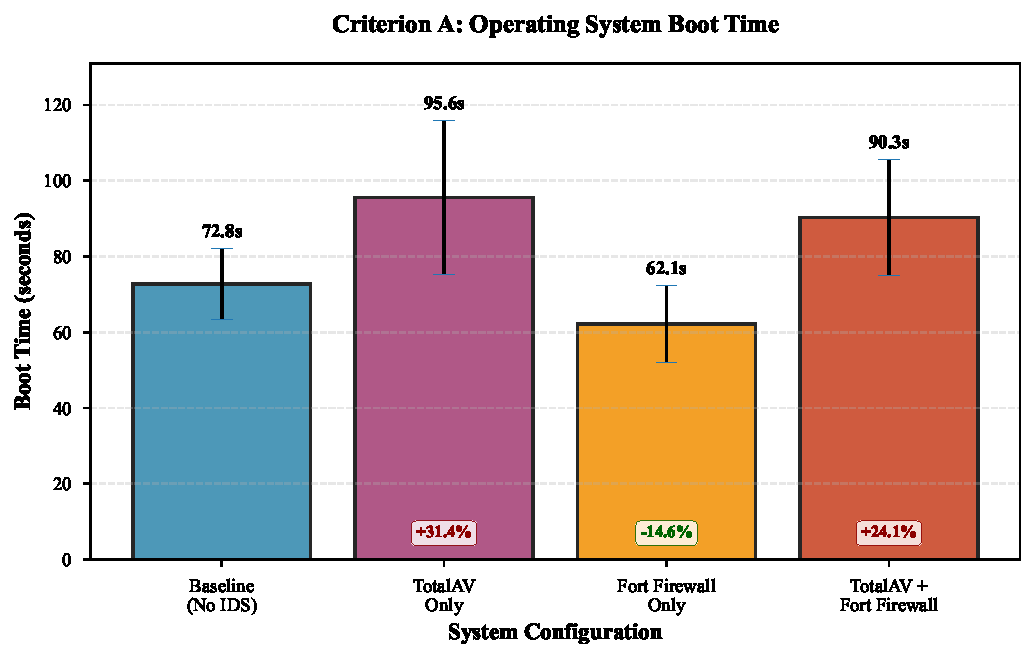
\includegraphics[width=0.85\textwidth]{figures/chart1_boot_time.pdf}
\caption{Operating System Boot Time Across Four IDS Configurations. Error bars represent standard deviation. Fort Firewall demonstrates unexpected 14.62\% improvement, while TotalAV imposes 31.39\% overhead.}
\label{fig:boot_time}
\end{figure}

\subsection{RAM Consumption}

\Cref{tab:ram_usage} shows memory usage patterns across configurations.

\begin{table}[htbp]
\caption{Memory Usage at Startup (MB)}
\label{tab:ram_usage}
\centering
\small
\begin{tabular}{@{}lrrr@{}}
\toprule
\textbf{Configuration} & \textbf{Mean} & \textbf{Std Dev} & \textbf{Overhead (\%)} \\
\midrule
Baseline & 2661.45 & 17.68 & --- \\
TotalAV Only & 3125.62 & 62.72 & \textbf{+17.44} (+464~MB) \\
Fort Firewall Only & 2700.77 & 85.89 & +1.48 (+39~MB) \\
Both IDS/IPS & 3203.13 & 140.61 & +20.35 (+542~MB) \\
\bottomrule
\end{tabular}
\end{table}

\textbf{Key Findings:} TotalAV consumed an additional 464~MB of RAM, which is typical for modern antivirus software that maintains threat databases in memory. Fort Firewall added only 39~MB, demonstrating efficient implementation. The combined overhead (542~MB) roughly approximates the sum of both components (464 + 39 = 503~MB), which indicates that the two systems maintain independent memory footprints (\Cref{fig:ram_usage}).

\begin{figure}[htbp]
\centering
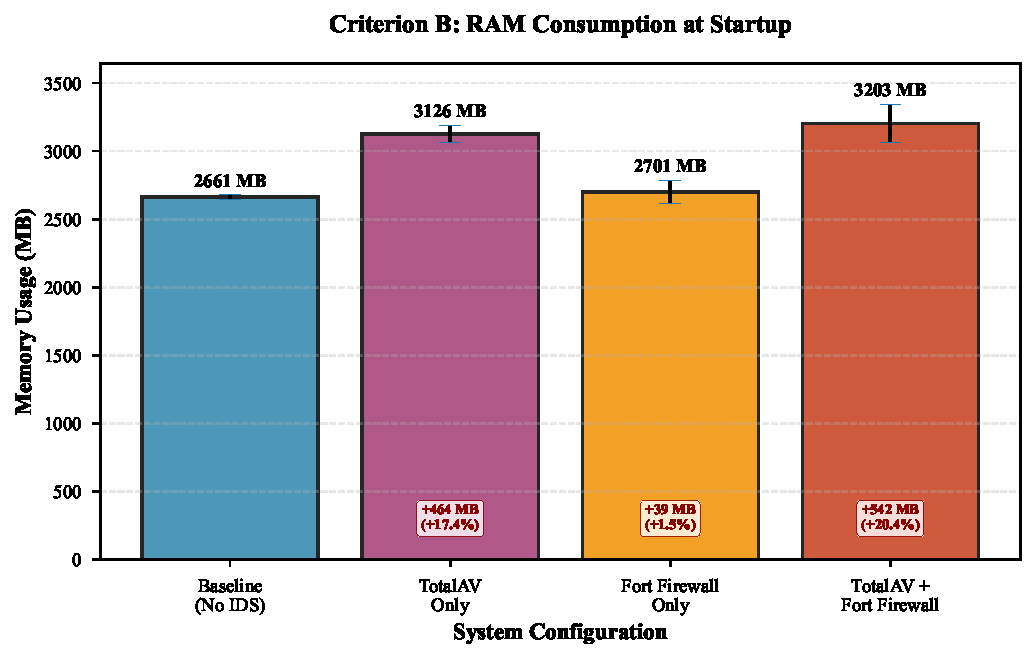
\includegraphics[width=0.85\textwidth]{figures/chart2_ram_usage.pdf}
\caption{RAM Consumption at System Startup. TotalAV accounts for majority of memory overhead (+464~MB), while Fort Firewall remains lightweight (+39~MB).}
\label{fig:ram_usage}
\end{figure}

\subsection{Process Count}

\Cref{tab:process_count} reveals minimal variation across configurations (147--152 processes).

\begin{table}[htbp]
\caption{Running Process Count}
\label{tab:process_count}
\centering
\small
\begin{tabular}{@{}lrrr@{}}
\toprule
\textbf{Configuration} & \textbf{Mean} & \textbf{Std Dev} & \textbf{Overhead (\%)} \\
\midrule
Baseline & 150.50 & 1.29 & --- \\
TotalAV Only & 147.33 & 2.08 & \textbf{-2.10}$^\dagger$ \\
Fort Firewall Only & 152.00 & 0.00 & +1.00 \\
Both IDS/IPS & 151.00 & 0.00 & +0.33 \\
\bottomrule
\multicolumn{4}{l}{\small $^\dagger$ TotalAV reduces process count through consolidation}
\end{tabular}
\end{table}

\textbf{Key Findings:} TotalAV reduced count by 2.10\%, suggesting efficient multi-threading or service consolidation. Low standard deviation indicates highly consistent measurements.

\subsection{Application Launch Performance}

\Cref{fig:app_launch} illustrates the most dramatic performance impact observed.

\begin{table}[htbp]
\caption{Application Launch Time (30 apps, seconds)}
\label{tab:app_launch}
\centering
\small
\begin{tabular}{@{}lrrr@{}}
\toprule
\textbf{Configuration} & \textbf{Mean} & \textbf{Std Dev} & \textbf{Overhead (\%)} \\
\midrule
Baseline & 14.46 & 2.89 & --- \\
TotalAV Only & 21.70 & 4.28 & \textbf{+50.05} \\
Fort Firewall Only & 11.85 & 2.24 & \textbf{-18.05}$^\dagger$ \\
Both IDS/IPS & 18.98 & 4.70 & +31.21 \\
\bottomrule
\multicolumn{4}{l}{\small $^\dagger$ Fort Firewall improves performance over baseline}
\end{tabular}
\end{table}

\textbf{Key Findings:} TotalAV imposed a severe 50.05\% penalty, increasing launch time from 14.46s to 21.70s. This indicates aggressive real-time executable scanning. In contrast, Fort Firewall actually improved performance by 18.05\% (down to 11.85s), consistent with the boot time improvements we observed. The combined deployment showed 31.21\% overhead—significantly less than TotalAV operating alone.

\begin{figure}[htbp]
\centering
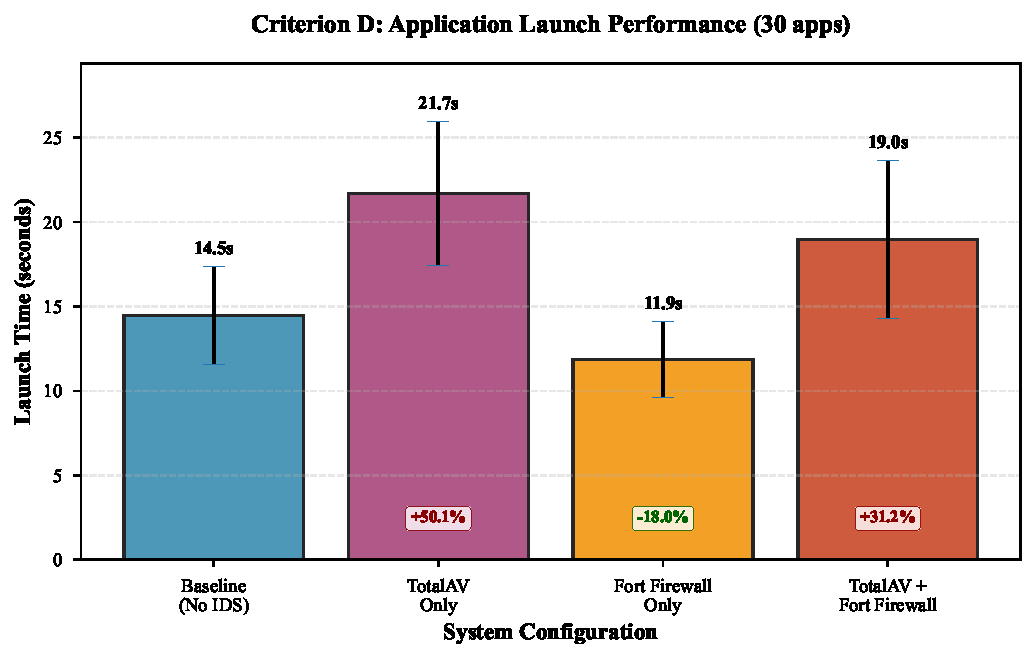
\includegraphics[width=0.85\textwidth]{figures/chart3_app_launch.pdf}
\caption{Application Launch Performance for 30 Applications. TotalAV imposes most severe overhead (+50.05\%), doubling launch time. Fort Firewall shows unexpected 18.05\% improvement.}
\label{fig:app_launch}
\end{figure}

\subsection{Network Performance}

\Cref{fig:network_performance} presents dual comparison of local (SMB) and remote (FTP) network transfers.

\begin{table}[htbp]
\caption{SMB Local Network Transfer (1~GB folder, MB/s)}
\label{tab:smb_transfer}
\centering
\small
\begin{tabular}{@{}lrrr@{}}
\toprule
\textbf{Configuration} & \textbf{Mean} & \textbf{Std Dev} & \textbf{Change (\%)} \\
\midrule
Baseline & 39.37 & 5.20 & --- \\
TotalAV Only & 31.79 & 6.72 & \textbf{-19.26} \\
Fort Firewall Only & 42.18 & 9.26 & \textbf{+7.14}$^\dagger$ \\
Both IDS/IPS & 35.91 & 6.56 & -8.80 \\
\bottomrule
\multicolumn{4}{l}{\small $^\dagger$ Fort Firewall exceeds baseline throughput}
\end{tabular}
\end{table}

\begin{table}[htbp]
\caption{FTP Remote Download (114.66~MB file, MB/s)}
\label{tab:ftp_download}
\centering
\small
\begin{tabular}{@{}lrrr@{}}
\toprule
\textbf{Configuration} & \textbf{Mean} & \textbf{Std Dev} & \textbf{Change (\%)} \\
\midrule
Baseline & 10.29 & 1.59 & --- \\
TotalAV Only & 9.18 & 1.32 & -10.83 \\
Fort Firewall Only & 8.50 & 1.95 & \textbf{-17.41} \\
Both IDS/IPS & 8.23 & 1.63 & \textbf{-20.02} \\
\bottomrule
\end{tabular}
\end{table}

\textbf{Key Findings:} TotalAV reduced SMB throughput by 19.26\% due to real-time file scanning. Fort Firewall improved SMB by 7.14\%, exceeding baseline through efficient packet processing. However, Fort Firewall imposed highest FTP penalty (-17.41\%), suggesting deep packet inspection overhead for external connections differs from local LAN behavior.

\begin{figure}[htbp]
\centering
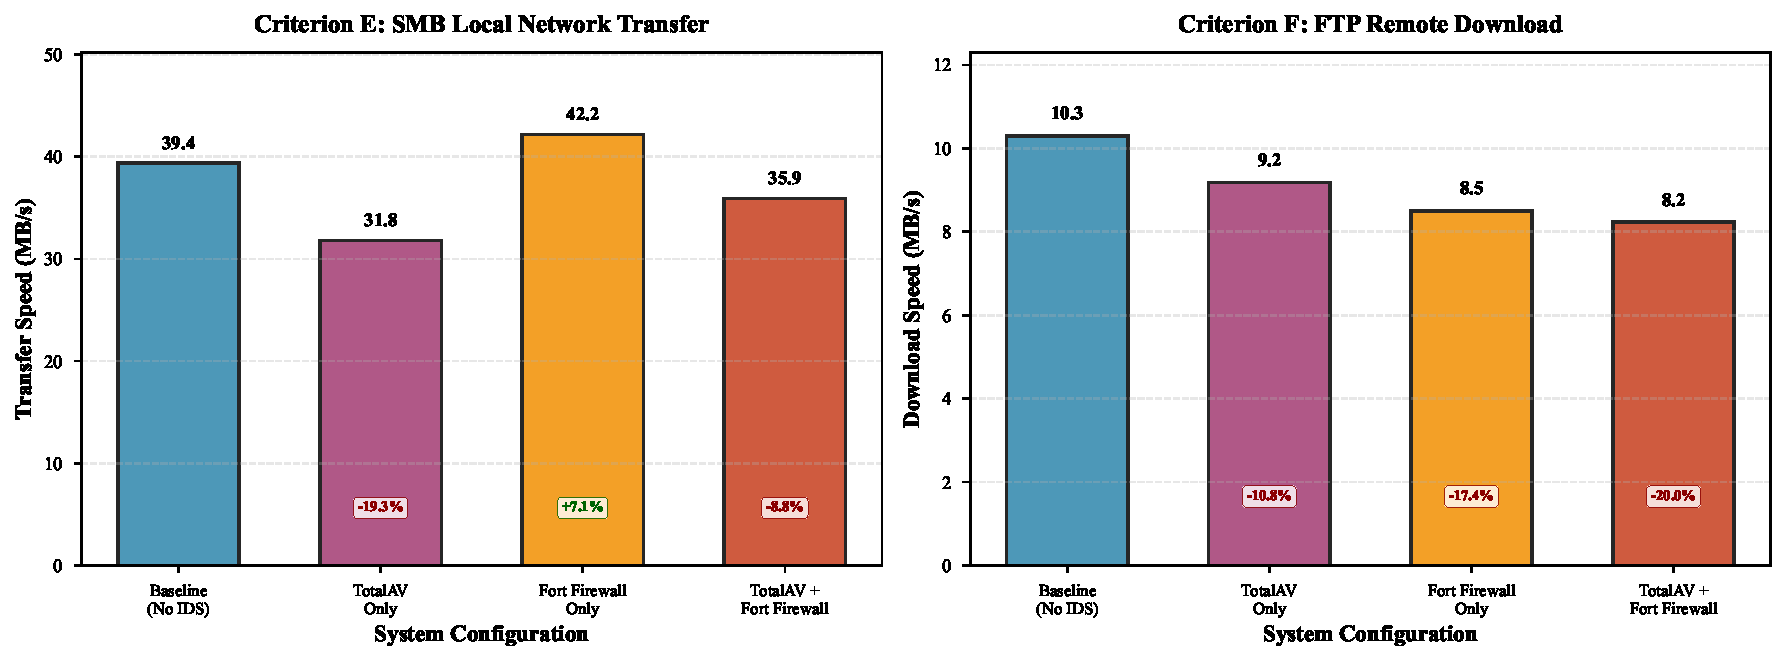
\includegraphics[width=\textwidth]{figures/chart4_network_performance.pdf}
\caption{Network Performance: SMB Local Transfer (left) and FTP Remote Download (right). Fort Firewall shows contrasting behavior: improving local network performance (+7.14\%) while degrading remote FTP (-17.41\%).}
\label{fig:network_performance}
\end{figure}

\subsection{Comprehensive Overview}

\Cref{fig:comprehensive_overhead} provides at-a-glance comparison across all metrics. \Cref{tab:comprehensive} summarizes overhead patterns.

\begin{table}[htbp]
\caption{Comprehensive Performance Overhead Comparison (\%)}
\label{tab:comprehensive}
\centering
\small
\begin{tabular}{@{}lrrr@{}}
\toprule
\textbf{Metric} & \textbf{TotalAV Only} & \textbf{Fort Firewall Only} & \textbf{Both IDS} \\
\midrule
Boot Time & +31.39 & \textbf{-14.62}$^\dagger$ & +24.09 \\
RAM Usage & +17.44 & +1.48 & +20.35 \\
Process Count & -2.10 & +1.00 & +0.33 \\
App Launch & +50.05 & \textbf{-18.05}$^\dagger$ & +31.21 \\
SMB Speed & -19.26 & \textbf{+7.14}$^\dagger$ & -8.80 \\
FTP Speed & -10.83 & -17.41 & -20.02 \\
\bottomrule
\multicolumn{4}{l}{\small $^\dagger$ Indicates performance improvement over baseline}
\end{tabular}
\end{table}

\begin{figure}[htbp]
\centering
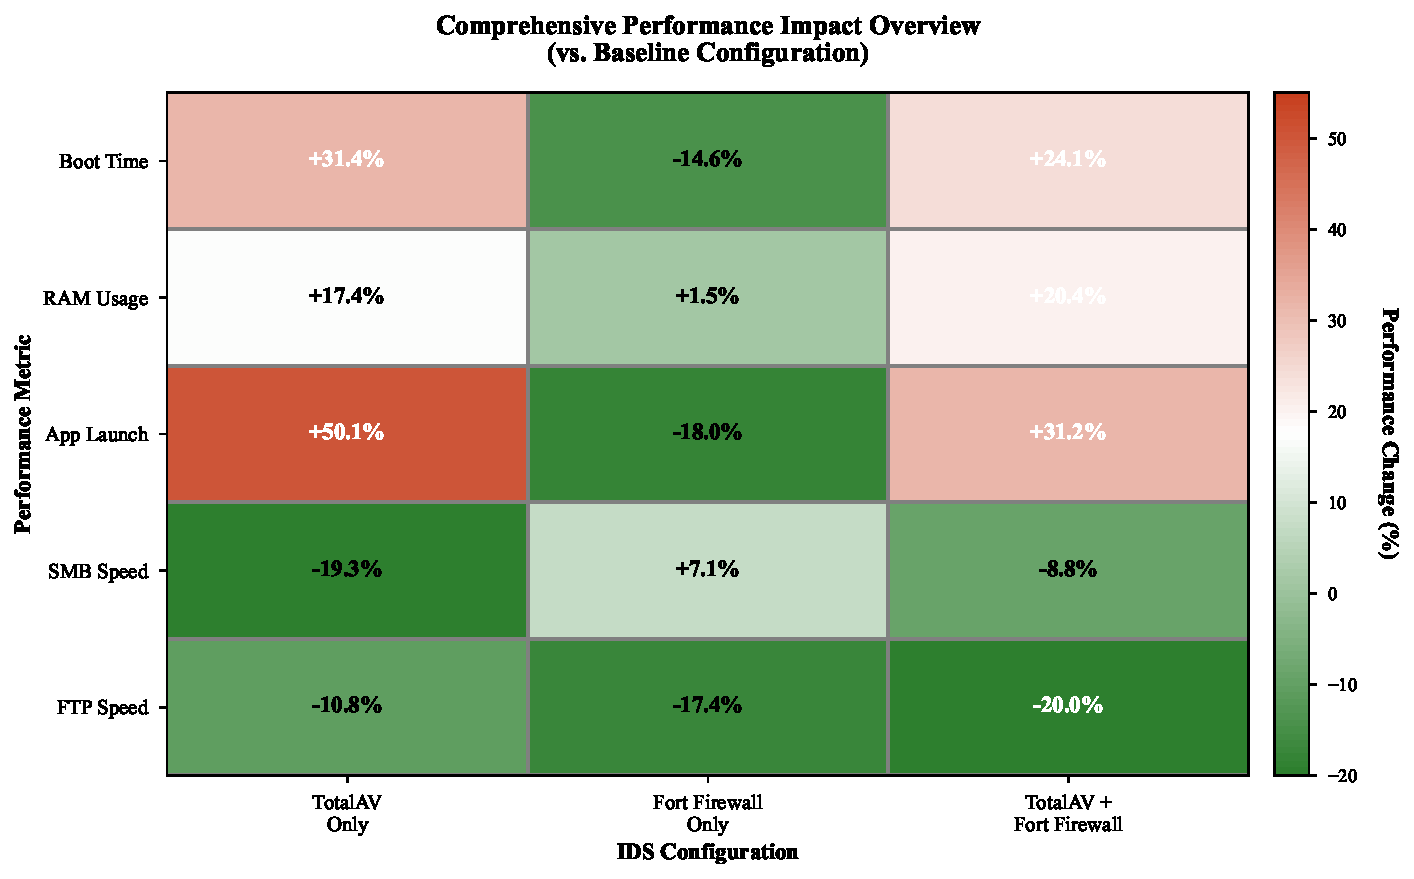
\includegraphics[width=0.95\textwidth]{figures/chart5_comprehensive_overhead.pdf}
\caption{Comprehensive Performance Impact Heatmap. Green indicates improvements, red indicates degradation. Fort Firewall shows unique optimization benefits across multiple metrics.}
\label{fig:comprehensive_overhead}
\end{figure}

\textbf{Overhead Categories:}
\begin{itemize}
\item \textbf{Severe ($>$20\%):} TotalAV boot (+31.39\%), app launch (+50.05\%), both FTP (-20.02\%)
\item \textbf{Moderate (10--20\%):} TotalAV RAM (+17.44\%), SMB (-19.26\%), Fort FTP (-17.41\%)
\item \textbf{Minimal ($<$10\%):} Fort RAM (+1.48\%), all process counts, both SMB (-8.80\%)
\item \textbf{Improved:} Fort boot (-14.62\%), app launch (-18.05\%), SMB (+7.14\%)
\end{itemize}

\section{Discussion}
\label{sec:discussion}

\subsection{TotalAV Performance Impact}

TotalAV demonstrated significant overhead across nearly all metrics, with the most severe impact on \textit{application launch} (+50.05\%). The doubling of launch time reflects the aggressive real-time executable scanning that prioritizes security over responsiveness. The 23-second \textit{boot delay} (from 72.76s to 95.60s) results from antivirus service initialization and signature database loading. \textit{SMB transfer} degradation (-19.26\%) stems from real-time on-access scanning that creates I/O bottlenecks. The 464~MB \textit{RAM overhead} (+17.44\%) is consistent with modern antivirus architectures that maintain resident threat databases and machine learning models.

\subsection{Fort Firewall Characteristics}

Fort Firewall exhibited unexpectedly positive performance across several metrics. The 10-second faster \textit{boot} and 2.6-second \textit{app launch} reduction likely result from efficient application whitelisting or reduced protocol stack overhead compared to Windows Firewall. The \textit{SMB throughput increase} (+7.14\%) indicates more efficient packet processing through optimized buffering. However, Fort Firewall imposed the highest \textit{FTP penalty} (-17.41\%), which suggests that deep packet inspection overhead for external traffic differs significantly from local LAN behavior.

\subsection{Combined Deployment Interactions}

\textbf{Subadditive Effects:} Boot time (24.09\% vs.\ expected 16.77\%) and app launch (31.21\% vs.\ expected 32.00\%) showed less overhead than the sum of individual components would suggest, which indicates shared Windows security APIs that reduce redundant system calls or Fort Firewall whitelisting TotalAV processes.

\textbf{Additive Effects:} RAM usage (20.35\% vs.\ expected 18.92\%) and FTP performance (-20.02\% vs.\ -28.24\%) remained largely independent, operating without significant interaction.

\subsection{Practical Recommendations}

\textbf{Performance-Critical Environments:} Fort Firewall demonstrated negligible or positive impact across most metrics except FTP. Organizations prioritizing performance may consider firewall-only deployments with network-based antivirus.

\textbf{Security-Critical Environments:} Full IDS deployment recommended despite 20--31\% overhead in time-sensitive operations. Combined 542~MB RAM overhead remains manageable on modern 8+ GB systems.

\textbf{Mobile/Battery-Constrained Devices:} 31\% boot penalty and 50\% app launch overhead may be unacceptable. Consider scheduled scanning during idle periods.

\textbf{Network-Intensive Workloads:} 19--20\% file transfer degradation may be problematic for file servers.

\subsection{Limitations}

VirtualBox introduces baseline performance penalty (estimated 5--15\%) compared to bare-metal installations. While this affects absolute values, relative comparisons remain valid. FTP tests showed higher variability due to Internet connection fluctuations. The 30-application test may not reflect enterprise applications with database connections and network authentication. Five iterations meet minimum statistical requirements, but larger samples would improve confidence intervals.

\section{Conclusion}
\label{sec:conclusion}

This study quantified TotalAV antivirus and Fort Firewall performance impact on Windows 11 through rigorous benchmarking. TotalAV imposed moderate-to-severe overhead (10.83--50.05\%), with most significant impact on application launch (+50.05\%) and boot time (+31.39\%). Fort Firewall demonstrated unexpected improvements in boot time (-14.62\%), application launch (-18.05\%), and local network transfers (+7.14\%), challenging assumptions about security software overhead.

Combined deployments showed subadditive effects in several metrics, suggesting architectural synergies. Network performance degraded across all IDS/IPS configurations (8.80--20.02%), indicating both antivirus I/O scanning and firewall packet inspection contribute independent bottlenecks.

Organizations must balance security requirements against performance through careful product selection and workload-appropriate deployment strategies. The quantitative metrics provided enable data-driven security policy development and capacity planning. Fort Firewall's performance improvements suggest opportunities for optimization in mainstream security products.

\subsubsection*{Acknowledgments}
We thank the open-source communities behind VirtualBox, BootRacer, and the LNCS LaTeX template for providing the tools that enabled this research.

\bibliographystyle{splncs04nat}
\bibliography{ids-paper}

\end{document}
